\documentclass[acmtog]{acmart}
\usepackage{graphicx}
\usepackage{subfigure}
\usepackage{natbib}
\usepackage{listings}
\usepackage{bm}
\usepackage{amsmath}

\definecolor{blve}{rgb}{0.3372549 , 0.61176471, 0.83921569}
\definecolor{gr33n}{rgb}{0.29019608, 0.7372549, 0.64705882}
\makeatletter
\lst@InstallKeywords k{class}{classstyle}\slshape{classstyle}{}ld
\makeatother
\lstset{ %
backgroundcolor=\color{white},   % choose the background color
basicstyle=\footnotesize\ttfamily,        % size of fonts used for the code
columns=fullflexible,
breaklines=true,                 % automatic line breaking only at whitespace
captionpos=b,                    % sets the caption-position to bottom
tabsize=4,
commentstyle=\color{mygreen},    % comment style
escapeinside={\%*}{*)},          % if you want to add LaTeX within your code
keywordstyle=\color{blue},       % keyword style
stringstyle=\color{mymauve}\ttfamily,     % string literal style
frame=single,
rulesepcolor=\color{red!20!green!20!blue!20},
% identifierstyle=\color{red},
language=c++,
}
\lstset{basicstyle=\ttfamily}

% Title portion
\title{Assignment 4: {Global Illumination}}

\author{Name:\quad Entropy-Fighter\\ student number:\ 2020533
\\email:\quad xxxx@shanghaitech.edu.cn}

% Document starts
\begin{document}
\maketitle

\vspace*{2 ex}

\section{Introduction}
\quad I do the must, bonus1, bonus2 and bonus4. In detail, I do the following things.
\begin{itemize}
\item (must)Path tracing with Monte Carlo integration, direct + indirect lighting (40 pts)
\item (must)Ideal diffuse BRDF and area light source (20 pts)
\item (must)Acceleration structure: BVH (30 pts)
\item (optional)The ideal specular or glossy specular BRDF (10 pts)
\item (optional)The translucent BRDF with refraction, e.g. glasses and diamonds. (10 pts)
\item (optional)Advanced BVH with higher performance. (20 pts)
\end{itemize}

\section{Implementation Details}
\subsection{Path tracing with Monte Carlo integration}
\quad This part is implemented in "integrator.cpp".
In this section, I complete the Integrator::render and Integrator::radiance methods. In general, to compute the radiance of each pixel in the image plane, I construct paths starting from the camera and compute the Monte-Carlo integration along these paths in order to solve the light transport equation. The iterative implementation of path tracing can be briefly summarized below.

\begin{figure}[h]
	\centering
	{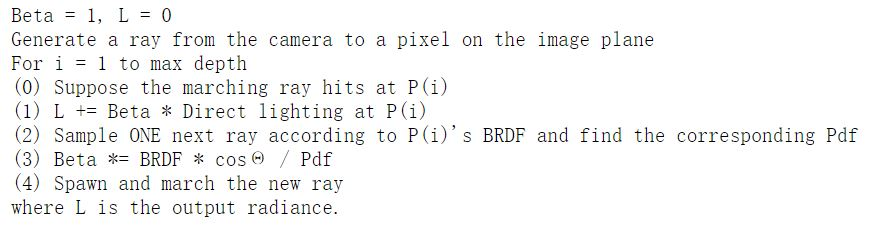
\includegraphics[width=9cm, height=4cm]{mc.JPG}}	
\end{figure}

The most important step of the above pseudo code is to calculate the direct lighting and indirect lighting. 


To calculate direct lighting, we need to sample the light source to generate a new ray. If the new ray is shadowed, we return. Otherwise, it it is not shadowed or blocked, we use the emission as $L_i$.

To calculate indirect lighting, we also need to sample to construct a new ray. 
After that, we need to test whether it hits the light.
If it hits the light, it means it is a direct lighting ray.
if it does not hit the light, it means it is not a direct lighting ray. Then we have to recursively calucate the radiance given the new ray.

\subsection{Ideal diffuse BRDF and area light source}
\quad This part is implemented in the "bsdf.cpp" and "light.cpp".

As for ideal diffuse BRDF, we use cos-weighted sampling. 

For function "evaluate", the return value should be $\frac{color}{\pi}$. For function "pdf", the return value should be $\frac{cos\theta}{\pi}$. 
For function "sample", we do the following things. 

We firstly sample uniformly by the sampler.
\begin{lstlisting}
	Vec2f eta = sampler.get2D();
\end{lstlisting}
Then we do the transformation from (x,y) to $(r,\theta_0)$.
The relation between them is $$r = \sqrt{x}, \theta_0 = 2\pi y $$
After that, we do the projection onto the unit hemisphere, which means transforming from $(r, \theta_0)$ to $(\theta, \phi)$
$$\sin\theta = \sqrt{x_1}$$ $$\phi = \theta_0 = 2\pi y $$
\begin{lstlisting}
	float theta = asin(sqrt(eta[0]));
  	float phi = 2 * PI * eta[1];
\end{lstlisting}
Since we have sphere coordinates, we can compute x, y, z.
$$ x = \sin\theta\cos\phi $$$$ y = \sin\theta\sin\phi $$$$ z = \cos\theta$$
\begin{lstlisting}
	Vec3f direction(sin(theta) * cos(phi), sin(theta) * sin(phi), cos(theta));
\end{lstlisting}
Finally, we need to transform from local space to world space.
\begin{lstlisting}
	Mat3f trans = Eigen::Quaternionf::FromTwoVectors(Vec3f(0.0f, 0.0f, 1.0f), interaction.normal).toRotationMatrix();
	Vec3f res = trans * direction;
	interaction.wo = res.normalized();
	return pdf(interaction);
\end{lstlisting}
After sampling, we can get the new ray.

As for area light source sampling, we just uniformly sample a point on the rectangle area. The pdf should be $\frac{1}{A}$. The code for "sample" function ia shown below.
\begin{lstlisting}
	Vec2f s = sampler.get2D();
 	Vec3f pos = position + Vec3f((s[0] - 0.5f) * size[0], 0.0f, size[1] * (s[1] - 0.5f));
    *pdf = 1 / float(size[0] * size[1]);
    interaction.wo = (pos - interaction.pos).normalized();
    return pos;
\end{lstlisting}

In "pdf" function, we do the things below. 
\begin{lstlisting}
	float cos= std::max(0.0f, -interaction.wo.dot(Vec3f(0, -1, 0)));
	float distance = (pos - interaction.pos).norm();
	return cos / distance / distance;
\end{lstlisting}
Solid angle's definition is $dw = \frac{dA \cos\theta^{'}}{distance^2}$, where 
$\cos\theta^{'} = w_i \cdot n_{l}$, $distance$ is the distance between position of samples on light an the intersection position. 
Now, our basic rendering function is $$L_o(x,w_o) = \int_{\Omega}L_i(p,w_i)f(p,w_i,w_o)\frac{\cos\theta\cos\theta^{'}}{distance^2}dA$$

\subsection{Acceleration structure: BVH}
\quad This part is implemented most in the "geometry.cpp". 
BVH is a new data structure whose name is bounding volume hierarchy.
Pbrt tells us that BVHs are an approach for ray intersection acceleration based on primitive subdivision, 
where the primitives are partitioned into a hierarchy of disjoint sets. All objects
are included in tree nodes of th bounding volume. The scene or each geometry/object can all be bounded by the recursive bounding volume.
\begin{itemize}
\item Organize objects into a tree
\item Group objects in the tree based on spatial relationships
\item Each node in the tree contains a bounding volume of all the objects below it
\end{itemize}

Here, we just do some simple introduction to how to construct, traverse a BVH tree. We would do some advanced implementations in the bonus part, and more details will be given in section 2.6. 
\begin{figure}[h]
	\centering
	\subfigure[construct]
	{
		\centering
		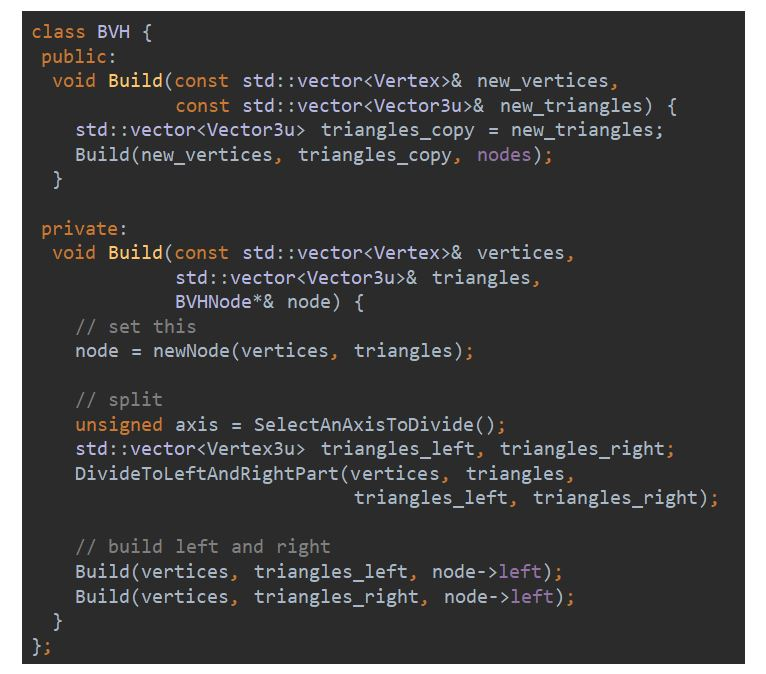
\includegraphics[width = 4cm]{simplebvh1.JPG}
	}
	\subfigure[raycast]
	{
		\centering
		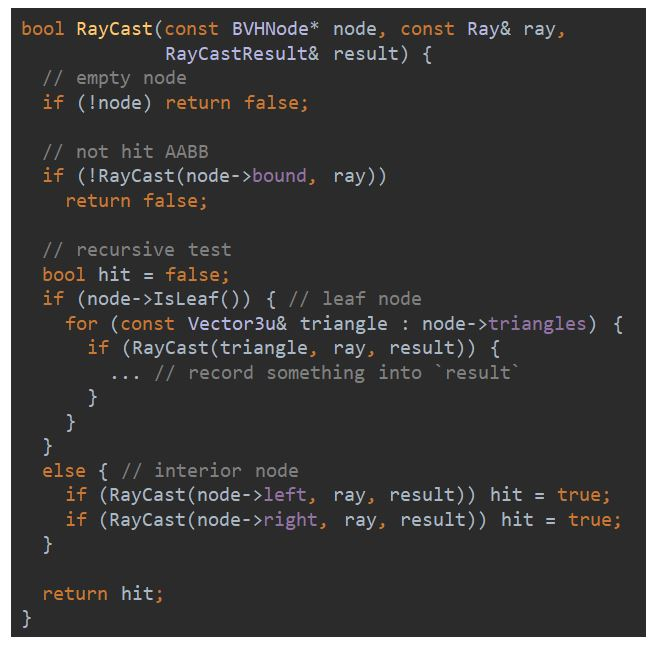
\includegraphics[width = 4cm]{simplebvh2.JPG}
	}
\end{figure}

\subsection{(optional)The ideal specular BRDF}
\quad This part is implemented in the "bsdf.cpp". 
Implementation of ideal specular BRDF is easy. we just sample the reflect light, which has a pdf of 1.
As for the "sample" function, the implementation is shown below.
\begin{lstlisting}
	float cos_theta = (-interaction.wi).dot(interaction.normal);
  	interaction.wo = (2 * cos_theta * interaction.normal + interaction.wi).normalized();
	return pdf(interaction);
\end{lstlisting}

\subsection{(optional)The translucent BRDF with refraction, e.g. glasses and diamonds}
Reference: I learn this part from https://www.pbr-book.org/3ed-2018/Reflection\_Models/Specular\_Reflection\_and\_Transmission.

\quad This part is implemented in the "bsdf.cpp". 
Implementation of the translucent BRDF with refraction is a bit harder than the ideal specular BRDF.
What we need to use here is snell law. 
$$\eta_1 \cdot \sin \theta_1 = \eta_2 \cdot \sin \theta_2$$

Snell law gives us the direction and also tells us that how the radiance changes when the ray goes
between different media with different indices of refraction.

In this part, we need to write a refract() function, which computes the refracted direction w. The core code(pbrt vesion) is given below.
\begin{lstlisting}
	inline bool Refract(const Vector3f &wi, const Normal3f &n, Float eta, Vector3f *wt) {
		Float cosThetaI = Dot(n, wi);
		Float sin2ThetaI = std::max(0.f, 1.f - cosThetaI * cosThetaI);
		Float sin2ThetaT = eta * eta * sin2ThetaI;
		if (sin2ThetaT >= 1) return false;

		Float cosThetaT = std::sqrt(1 - sin2ThetaT);

		*wt = eta * -wi + (eta * cosThetaI - cosThetaT) * Vector3f(n);
		return true;
	}
\end{lstlisting}
As for the "sample" function, it is similar to the specular part, but we need to consider the refract. The core part of the implementation is shown below.
\begin{lstlisting}
	bool refracted = Refract(-interaction.wi, interaction.normal, etaI / etaT, &interaction.wo);
	if(!refracted){
	  interaction.wo = (2 * cos_theta * interaction.normal + interaction.wi).normalized();
	}
	return pdf(interaction);
\end{lstlisting}
\subsection{(optional)Advanced BVH with higher performance(using SAH)}
Reference: I learn this part from https://medium.com/@bromanz/how-to-create-awesome-accelerators-the-surface-area-heuristic-e14b5dec6160 
and https://blog.csdn.net/weixin\_44176696/article/details/118655688

\quad This part is implemented in the "geometry.cpp". In this part, SAH is used to achieve better performance.
MacDonald and Booth proposed the SAH. It predicts the cost of a defined split position on a per-node basis. 
The model states that:
\begin{figure}[h]
	\centering
	{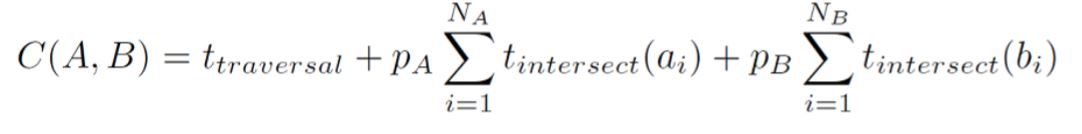
\includegraphics[width=8cm]{sah1.JPG}}	
\end{figure}
\begin{itemize}
	\item C(A, B) is the cost for splitting a node into volumes A and B
	\item t\_traversal is the time to traverse an interior node
	\item p\_A and p\_B are the probabilities that the ray passes through the volumes A and B
	\item N\_A and N\_B are the number of triangles in volumes A and B
	\item a\_i and b\_i are the ith triangle in volumes A and B
	\item t\_intersect is the cost for one ray-triangle intersection.
\end{itemize}
We can compute p\_A and p\_B as:
\begin{figure}[h]
	\centering
	{
\includegraphics[width=8cm]{sah2.JPG}}	
\end{figure}

\begin{itemize}
\item S\_C and S\_P are the surface areas of volumes C and P (We can simply compute the surface area of a node by summing all faces of a node)
\item p(C|P) is the conditional probability that a random ray passing through P will also pass through C, given that C is a convex volume in another convex volume P.
\end{itemize}

With this formula, the SAH rewards many triangles in tight boxes which are not likely to get pierced by a ray.
We can compute the SAH for various split positions. Then, we select the one with the lowest cost. We can receive possible split positions by taking triangle bounds into consideration. Another method is called binning. It defines a certain amount of linearly distributed positions over an axis. 

In our case, for n triangle meshes, we firstly traverse all the possible cases to
find the split method with least. And we should try every axis, namely the x
axis, y axis and z axis. After each traversal, we update and continue to do such things recursively.
There exists a small problem. We need to calculate the AABB bounding box about n times. If we traverse the interval to find the maximum value to build the bounding box every time, the efficiency of tree building will be very low. We have a little trick, using the idea of prefix to pre-calculate the maximum and minimum xyz values of the interval [l, i], [i+1, r], and then spend O(1) time to query each time.
\section{Results}
% pictures should be in
\begin{figure}[h]
	\centering
	{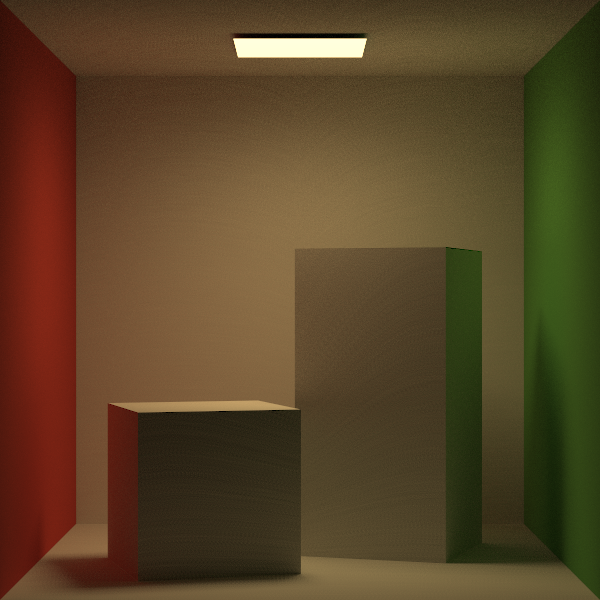
\includegraphics[width=8cm]{result0.png}}	
	\caption{simple}
\end{figure}
\begin{figure}[h]
	\centering
	{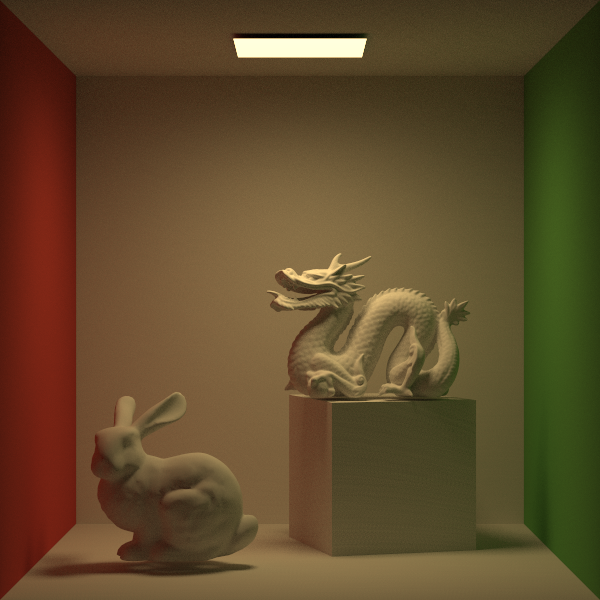
\includegraphics[width=8cm]{result1.png}}	
	\caption{large mesh}
\end{figure}
\begin{figure}[h]
	\centering
	{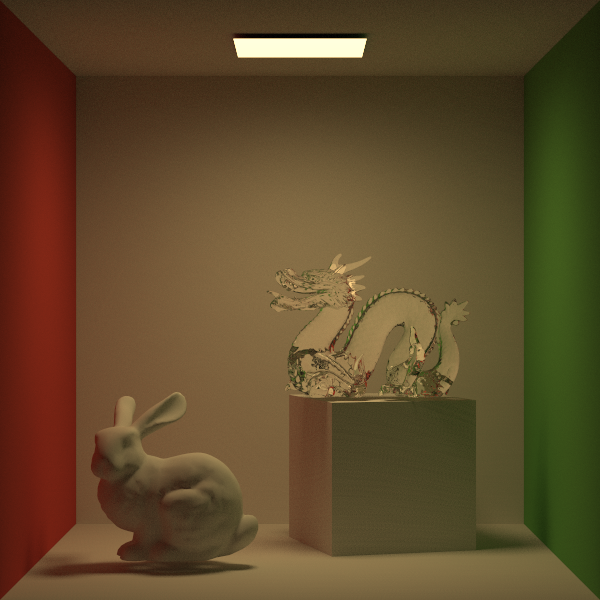
\includegraphics[width=8cm]{result2.png}}
	\caption{translucent}	
\end{figure}
\begin{figure}[h]
	\centering
	{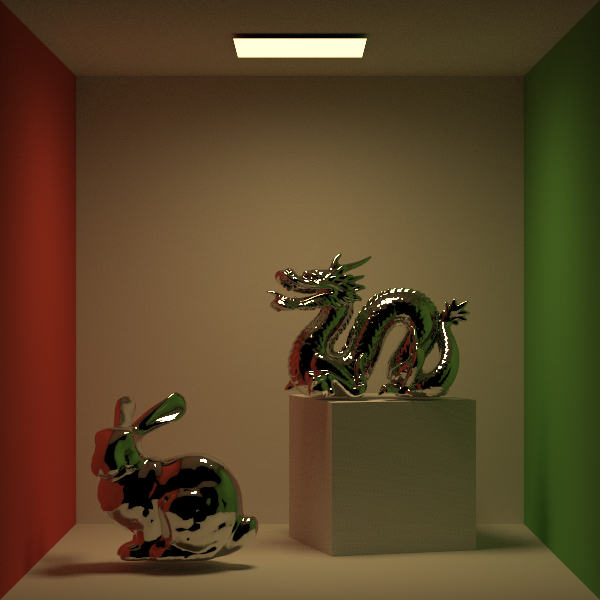
\includegraphics[width=8cm]{result.png}}
	\caption{specular}	
\end{figure}
\end{document}
